\documentclass[sigconf]{acmart}

\usepackage{graphicx}
\usepackage{pgfplots}

\usepackage{amssymb}
\usepackage{amsmath}
\usepackage{booktabs}

\usepackage{enumitem}
\usepackage{marginnote}
\setlength{\marginparwidth}{15mm}
\setlength{\marginparsep}{1mm}
\definecolor{darkblue}{rgb}{0.0,0.0,0.3}
\newcommand\todo[1]{\textcolor{blue}{[TODO: #1]}}
\newcommand\TODO[1]{\textcolor{blue}{\small [#1]}}
\newcommand\TODOM[1]{\marginpar{\color{blue}\renewcommand{\baselinestretch}{0.8}\tiny\tolerance=100000\hyphenpenalty=0\raggedright #1}}

% Input Graph

\def\iG{G}  % Input graph
\def\iV{V}  % Input nodes
\def\iv{v}  % Input node
\def\iE{E}  % Input edges
\def\ie{e}  % Input edge

% Drawing

\newcommand\drawing[1]{\mathcal{D}_{#1}}  % Drawing of graph
\newcommand\initdrawing[1]{\drawing{#1}^*}  % Drawing of graph

\def\drawingcurvesym{c}  % edge curve part of drawing
\def\drawingpossym{p}    % node position part of drawing

\newcommand\drawingcurve[1]{\drawingcurvesym(#1)}  % Drawing curve of argument edge
\newcommand\drawingpos[1]{\drawingpossym(#1)}  % Drawing pos urve of argument node

% Grid

\def\gScale{C}
\def\gmind{\hat d}


% Octilinear grid graph

\def\gG{\Gamma}  % Grid graph
\def\gV{\Psi}  % Grid graph nodes
\def\gv{\psi}  % Grid graph node
\def\gE{\Omega}  % v edges
\def\ge{\omega}  % Grid graph edge

\newcommand\ggv[2]{\gv_{#1, #2}}  % Grid node at #1, #2
\newcommand\gpv[3]{\gv_{#1, #2}^{#3}}  % Port #3 node at #1, #2
\newcommand\gse[3]{\ge_{#1, #2}^{#3}}  % Sink edge #3 node at #1, #2
\newcommand\gbe[4]{\ge_{#1, #2}^{#3, #4}}  % Bend edge for angle #4 at port #3 at node at #1, #2

\def\gPath{p}    % path on grid graph
\def\gPathOcti{p'}    % path on octilinear grid graph

\newcommand\gPturn[1]{c_{#1}}  % Turn penalty
\newcommand\gPturnEdge[1]{c'_{#1}}  % Turn penalty
\def\gHopcost{c_h}    % Hop cost in grid graph
\def\gHopcostOcti{c'_h}    % Hop cost in grid graph
\def\gSinkcost{c_s}    % Hop cost in grid graph
\newcommand\gPcost[1]{c(#1)}  % Path cost
\newcommand\gPcostOcti[1]{c'(#1)}  % Octilinear path cost

% ILP

\newcommand\gvused[2]{x_{#1#2}}	% bin. decision variable whether grid node #1 is assigned to input node #2
\newcommand\geused[2]{x_{#1#2}}	% bin. decision variable whether grid edge #1 is used be input edge #2

\newcommand\dir[2]{\delta_{#1#2}}	% variable telling the direction of edge #2 at node #1
\newcommand\dirdiff[2]{\Delta_{#1#2}}	% variable telling the direction difference of edge #1 and edge #2

\newcommand\bend[3]{\Delta_{#1#2}^{#3}}	% variable telling the direction difference of edge #1 and edge #2

\def\ldeg{\text{ldeg}}

\usepackage{tikz}
\usetikzlibrary{calc,trees,positioning,arrows,chains,shapes.geometric,%
  decorations.pathreplacing,decorations.pathmorphing,shapes,%
  matrix,shapes.symbols,plotmarks,decorations.markings,shadows}

\DeclareMathOperator{\atantwo}{atan2}

% Copyright
%\setcopyright{none}
%\setcopyright{acmcopyright}
%\setcopyright{acmlicensed}
\setcopyright{rightsretained}
%\setcopyright{usgov}
%\setcopyright{usgovmixed}
%\setcopyright{cagov}
%\setcopyright{cagovmixed}

% DOI
%\acmDOI{10.475/123_4}

% ISBN
%\acmISBN{123-4567-24-567/08/06}

%Conference
\acmConference[Some conference]{Some conference}{Some date}{Somewhere}
\acmYear{2021}
\copyrightyear{2021}

\renewcommand{\topfraction}{0.96}
\renewcommand{\textfraction}{0.01}
\renewcommand{\floatpagefraction}{0.96}

\def\Hms{\makebox[1.6mm][l]{\hspace{0.2mm}\footnotesize ms}}
\def\Hs{\makebox[1.6mm][l]{\hspace{0.2mm}\footnotesize s}}
\def\Hk{\makebox[1.6mm][l]{\hspace{0.2mm}\footnotesize k}}
\def\Hm{\makebox[1.6mm][l]{\hspace{0.2mm}\footnotesize m}}
\def\Hh{\makebox[1.6mm][l]{\hspace{0.2mm}\footnotesize h}}
\def\Hhline{\\[.7mm]\hline}

\makeatletter
\DeclareRobustCommand*\cal{\@fontswitch\relax\mathcal}
\makeatother

\DeclareMathOperator*{\argmin}{\arg\!\min}
\DeclareMathOperator*{\argmax}{\arg\!\max}
\DeclareMathOperator*{\TED}{TED}
\DeclareMathOperator*{\lev}{lev}

\begin{document}
\title{Metro Maps on Flexible Base Grids}

\begin{abstract}
We show that a previously developed method of drawing metro-maps on octilinear grid graphs can be used to draw metro maps following arbitrary base grids.
We experiment with several types of such base grids: ortho-radial grids, octilinear quad trees, octilinear Hanan grids (which we introduce in this work) and TODO.
Our interest is threefold:
first, we want to speed up the original approach by using a simplified base grid which still guarantees octilinearity.
Second, we are interested in the capability of the original approach to render maps which are not octilinear, but for example ortho-radial.
Last, we would like our approach to automatically adapt to the local node densities of the input graph.
We also show how quad trees can be used to enlarge high-density areas into otherwise empty areas.
\end{abstract}

\maketitle

\section{Introduction}

Drawing generalized metro maps is a well-studied topic.
Usually, the goal is to produce octilinear maps in which all edge segments have an orientation which is a multiple of 45 degrees.
In \cite{TODO}, an approach was described to render such maps with an arbitrary number of edge bends by routing the edges of the input graph in a special octilinear grid graph (the base grid) in which line bends where penalized.
This approach can be optimized exactly via an Integer Linear Program, or by a fast approximation method.
In this work, we want to study how this approach behaves when different kinds of base grids are used.
Our experiments will show the following:
(1) In the context of octilinear drawings, the size of the octilinear base grid graph can be greatly reduced with only minimal impact on the solution quality. To achieve this, we introduce the concept of an octilinear Hanan grid.
This is motivated by the well-known fact that a (regular) Hanan grid for a set of points $P$ containes an optimal rectilinear Steiner Tree for $P$.
(2) The approach is able to render ortho-radial, triangular or hexagonal metro maps with only minor modifications by using corresponding base grids.
(3) If quad trees are used as base grids, the metro map density can be dynamically adjusted to local input graph densities. Quad trees can also be used to enlarge high-density into neighboring low-density areas.

We use the following notation:
Our input is an undirected labeled graph $\iG = (\iV, \iE, L)$.
$\iV$ may be understood as stations but may also contain non-station intersections.
The edges $\iE$ are connections between nodes labeled with lines $L(e) \subseteq \mathcal{L}$ traveling through them.
We then search for a drawing $\mathcal{D}(G)$ of $G$ that resembles a metro map.

\begin{figure}
    \centering
	\vspace{-0.6cm}
	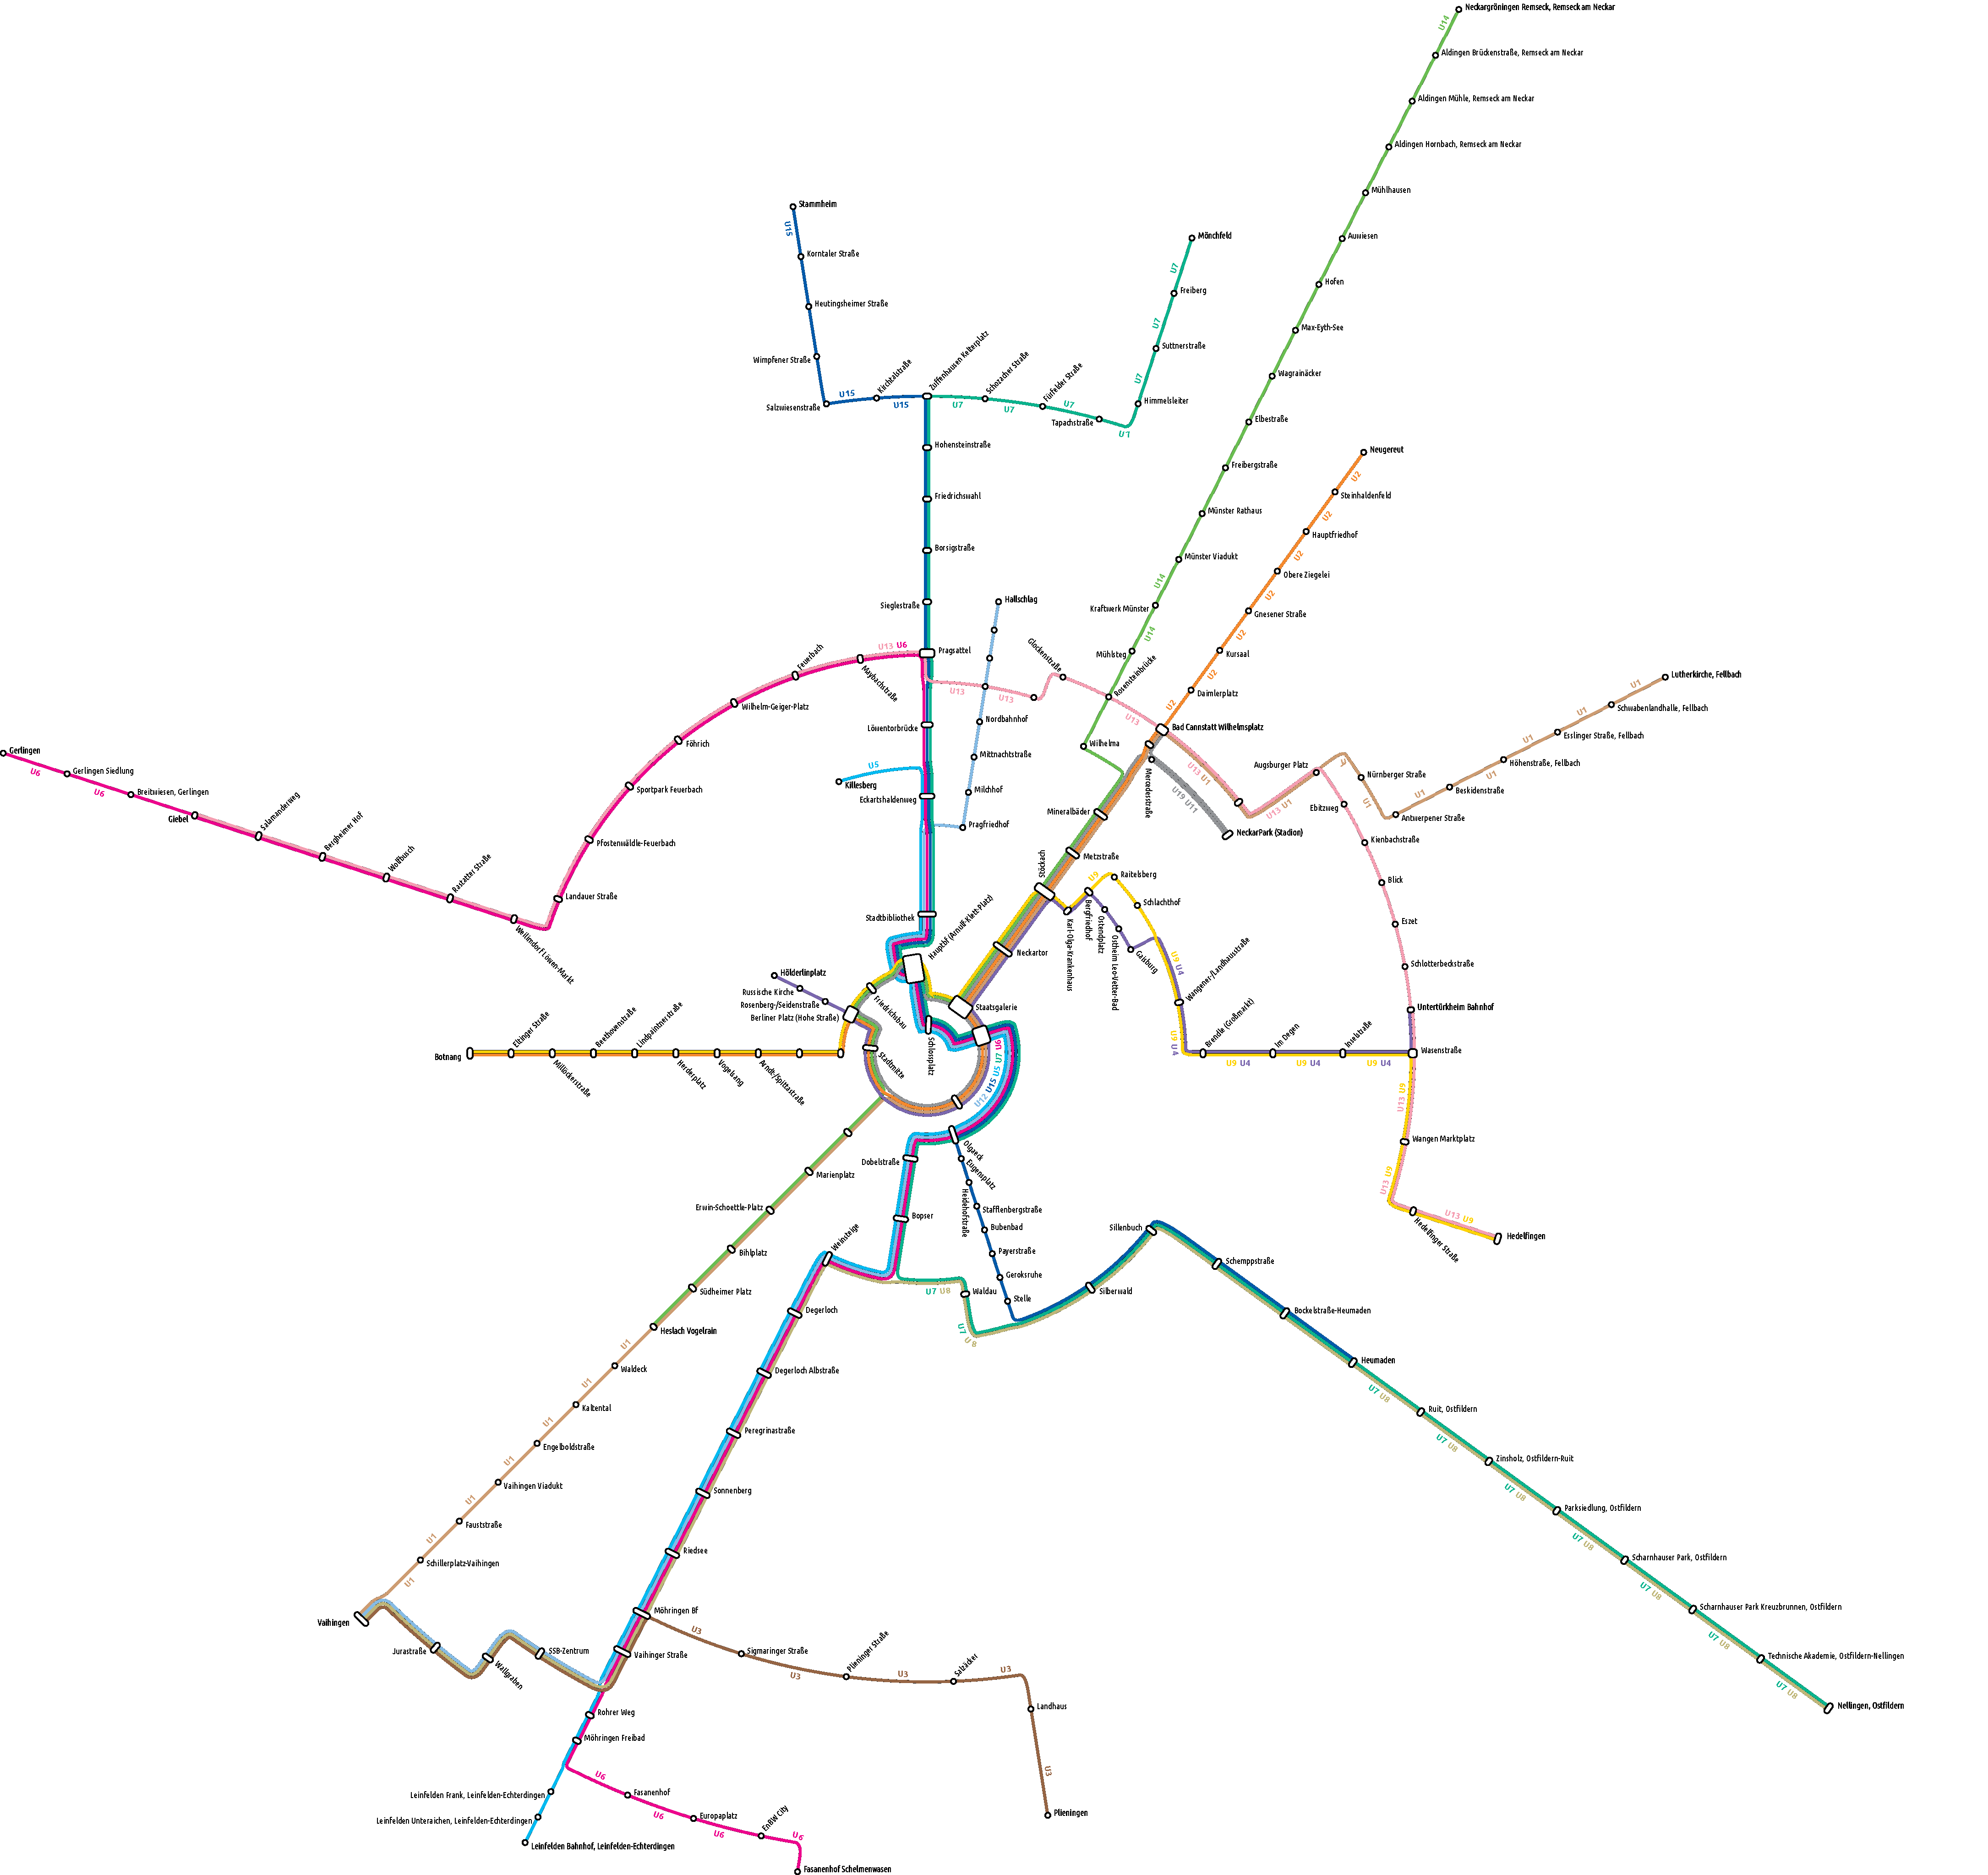
\includegraphics[width=0.47\textwidth]{figures2/stuttgart-ortho.pdf}
	\caption{The Stuttgart light rail network rendered in an ortho-radial fashion by our approach.}
	\label{FIG:stuttgart}
\end{figure}

\subsection{Related Work}
\label{SEC:related}

\TODO{describe the original approach}
\TODO{other related work, especially recent work on orthoradial metro maps, but also bezier curve based maps}

\subsection{Metro Maps on Grid Graphs}

The method described in \cite{TODO} first builds an octilinear grid graph with the size of the bounding box of the input graph $G$.
The grid cell size can be chosen freely.
In \cite{TODO}, it was observed that the average distance between adjacent nodes in the input graph works well in practice.
The optimal drawing is then constructed by routing all input edges in this octilinear grid graph, with the restriction that no routed edge may cross another routed edge.
The assignment of input nodes to grid nodes is unrestricted, but a larger geographical distance to the original position is penalized.
To be able to penalize line bends in the final drawing, grid nodes were extended by so-called port nodes, which made it possible to add penalty costs to bends.
The modelling of these line bend costs is similar to the modelling of turn costs in transportation networks, but does not require a directed graph.
Additionally, the circular ordering of outgoing edges in the input graph were required to remain the same in the final drawing.

\begin{figure}
    \centering
	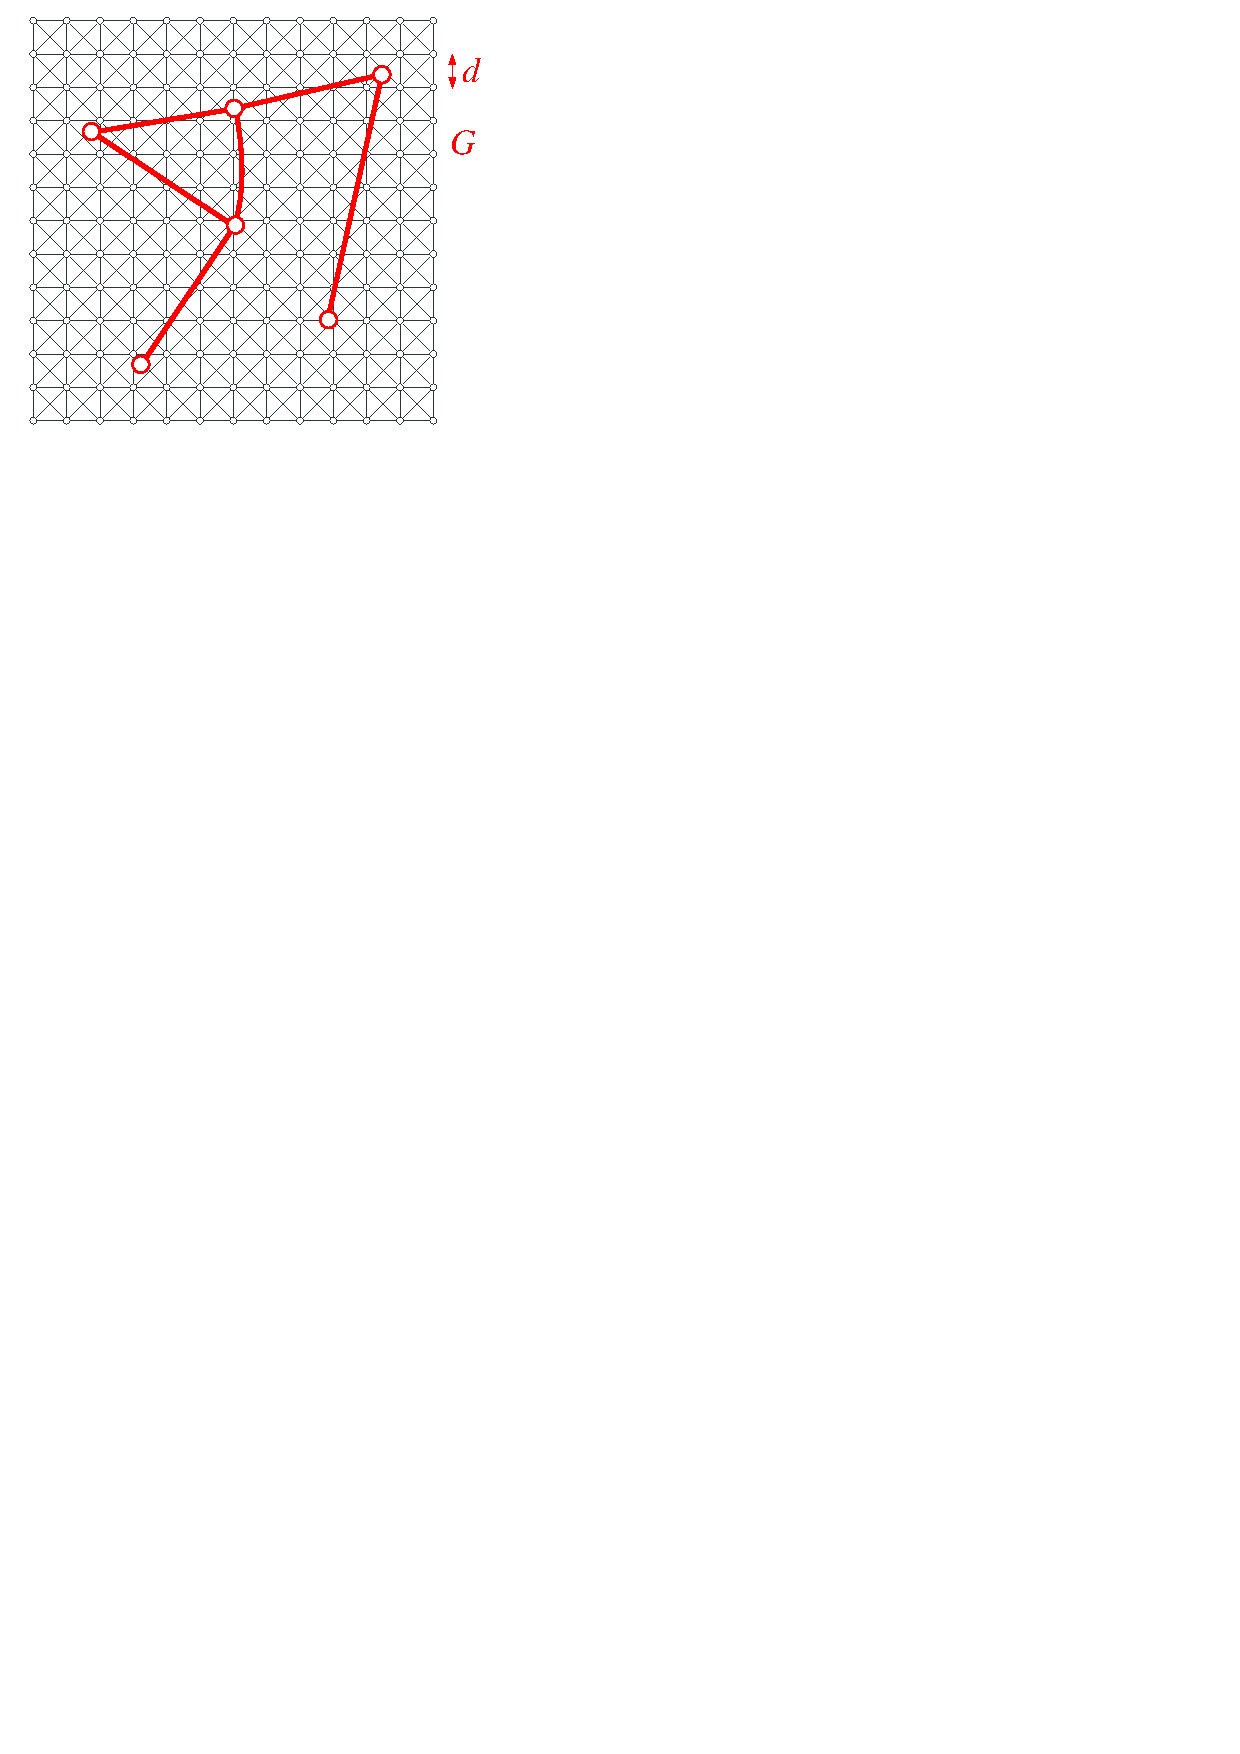
\includegraphics[width=0.24\textwidth]{figures2/grid2.pdf}
	\hfill
	\includegraphics[width=0.2257\textwidth,trim=0 0 15 0, clip, page=2]{figures2/grid2.pdf}
	\caption{TODO}
	\label{FIG:griddrawing}
\end{figure}

As an ILP based solution to compute the globally optimal drawing proved to be too slow, an approximate approach was developed in which edges we routed explicitely through the grid graph by Dijkstras algorithm.
As a polishing step, a local search was added.

\TODO{mention missing enlargement of dense areas}

\section{Node Splitting}

Naturally, octilinear metro maps can only be drawn for input graphs with a maximum node degree less than 9.
Real-world transportation networks typically satisfy this requirement.
However, orthoradial metro maps require a maximum node degree of 4.
Triangular maps require a maximum node degree of only 3.
As node degrees larger than 4 are still common in real-world transit networks, this problem has to be addressed prior to rendering such maps.

\begin{figure}
    \centering
	\hfill
	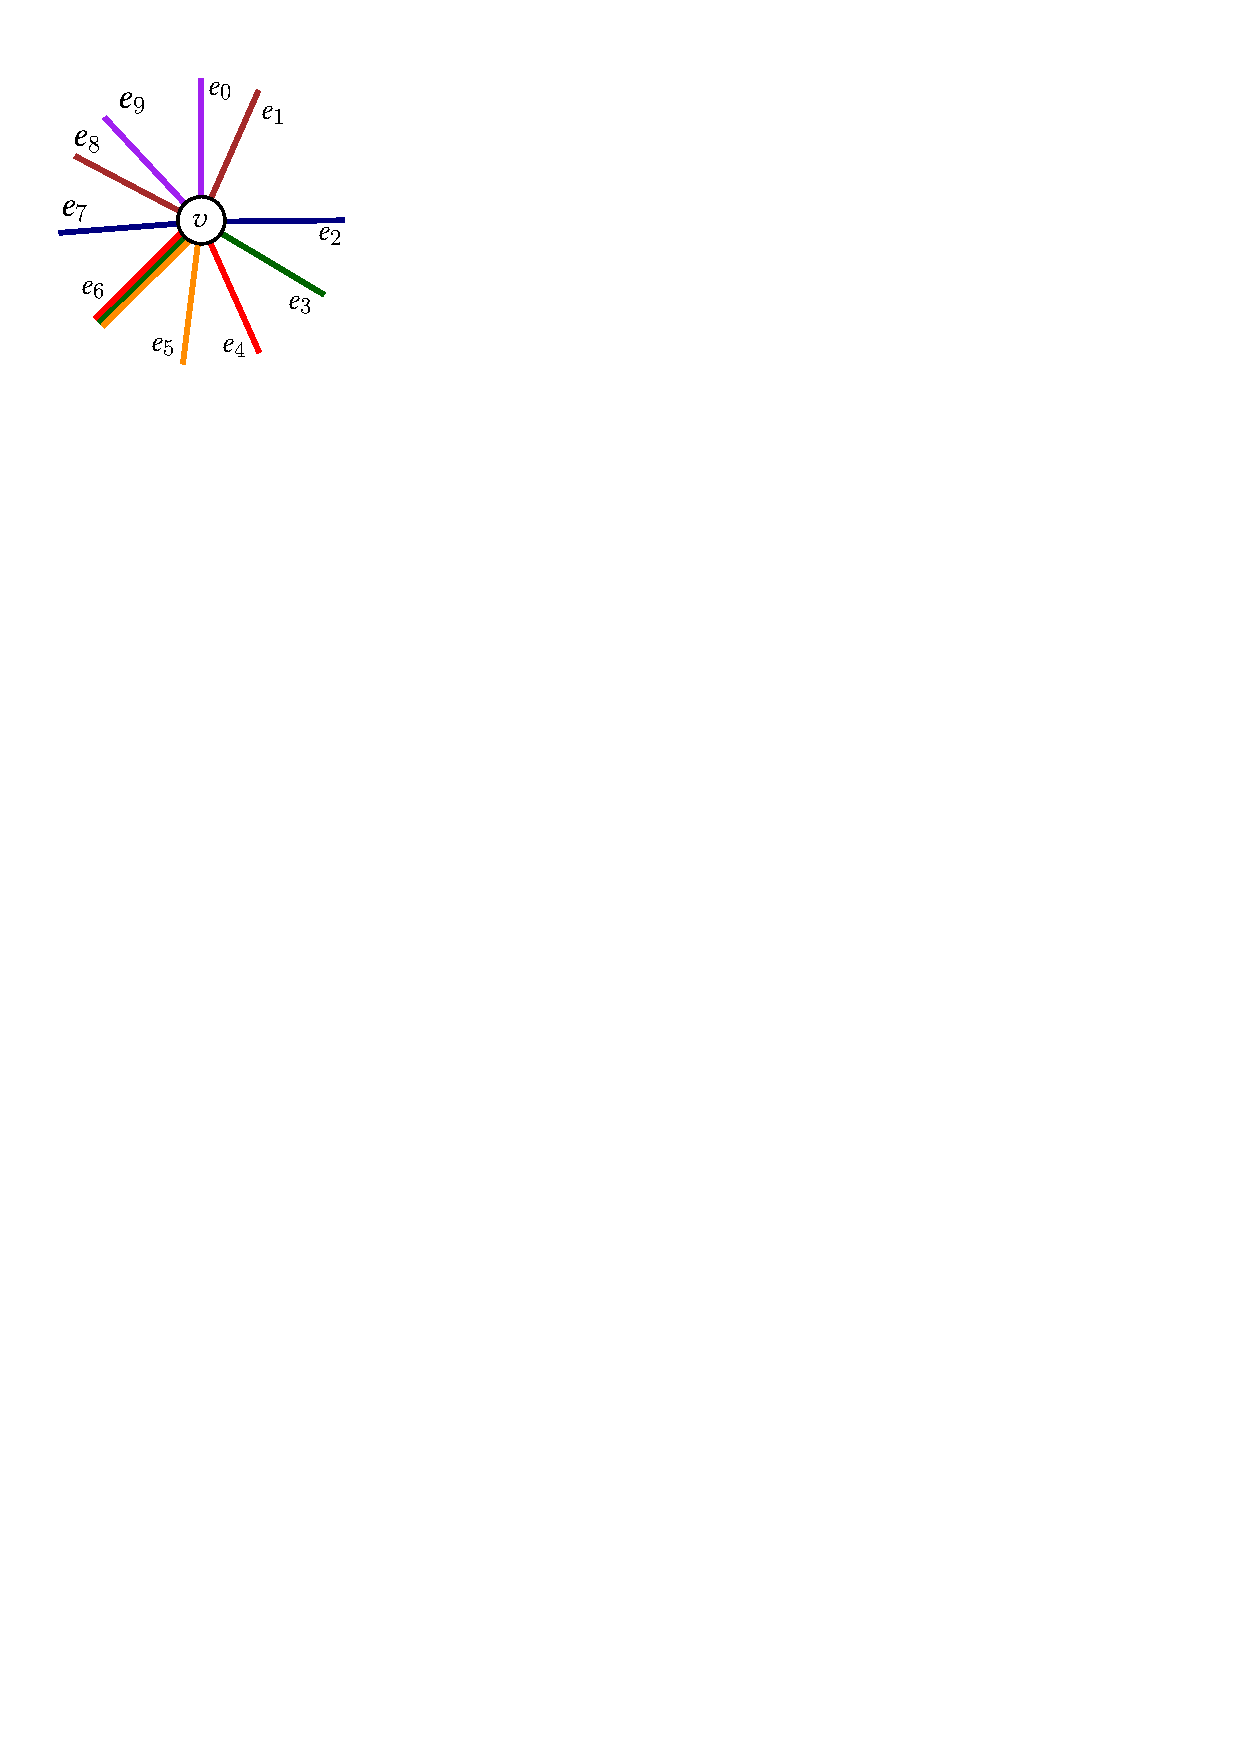
\includegraphics[width=0.18\textwidth]{figures2/nodesplit.pdf}
	\hfill
	\includegraphics[width=0.18\textwidth,page=2]{figures2/nodesplit.pdf}
	\hfill
	\caption{Left: Node $v$ in an input line graph has a degree of 6, making it impossible to render the graph in an orthoradial fashion. Right: We keep the first (in clockwise order) 3 adjacent edges of $v$, combine the lines of the remaining edges $e_4$, $e_5$ and $e_6$ into a single new edge $f$ and connect it to a new non-station node $v'$.}
	\label{FIG:orthoradgrid}
\end{figure}

A simple approach is depicted in Figure~\ref{TODO}.
Given a maximum node degree $D$, a node $v$ with $\deg(v) > D$ and indicent edges $e_1 \dots e_{\deg(v)}$, we remove edges $e_{D+1} \dots e_{\deg(v)}$ from $v$ and add them to the new node $v'$.
An additional edge $f$ is added between $v'$ and $v$ with $L(f) = \bigcup_{e_{D+1} \dots e_{\deg(v)}} L(e)$.
If we still have $\deg(v') > D$, we repeat to process for $v'$.
Note that while Figure~\ref{TODO} depicts $v'$ with a different position than $v'$, this position will remain the same as $v$ in the modified input graph to not distort displacement penalties during the metro map rendering.

\section{Octilinear Hanan Grid}

Given a set of two-dimensional points $P$, the Hanan grid $H(P)$ is a graph that can be constructed in the following way:
(1) Draw vertical and horizontal lines through each $p \in P$.
(2) Where these lines intersect, add vertices.
A Hanan grid $H(P)$ contains a minimum rectilinear Steiner tree for $P$.
As rectilinear Steiner trees are slightly related to rectilinear Metro Maps, it seems worthwhile to evaluate they applicability to grid-based Metro Map drawing.
In particular, given the relative sparsity of a Hanan grid when compared to a full grid, they have the potential to speed up the time needed to generate such drawings.

\begin{figure}
    \centering
	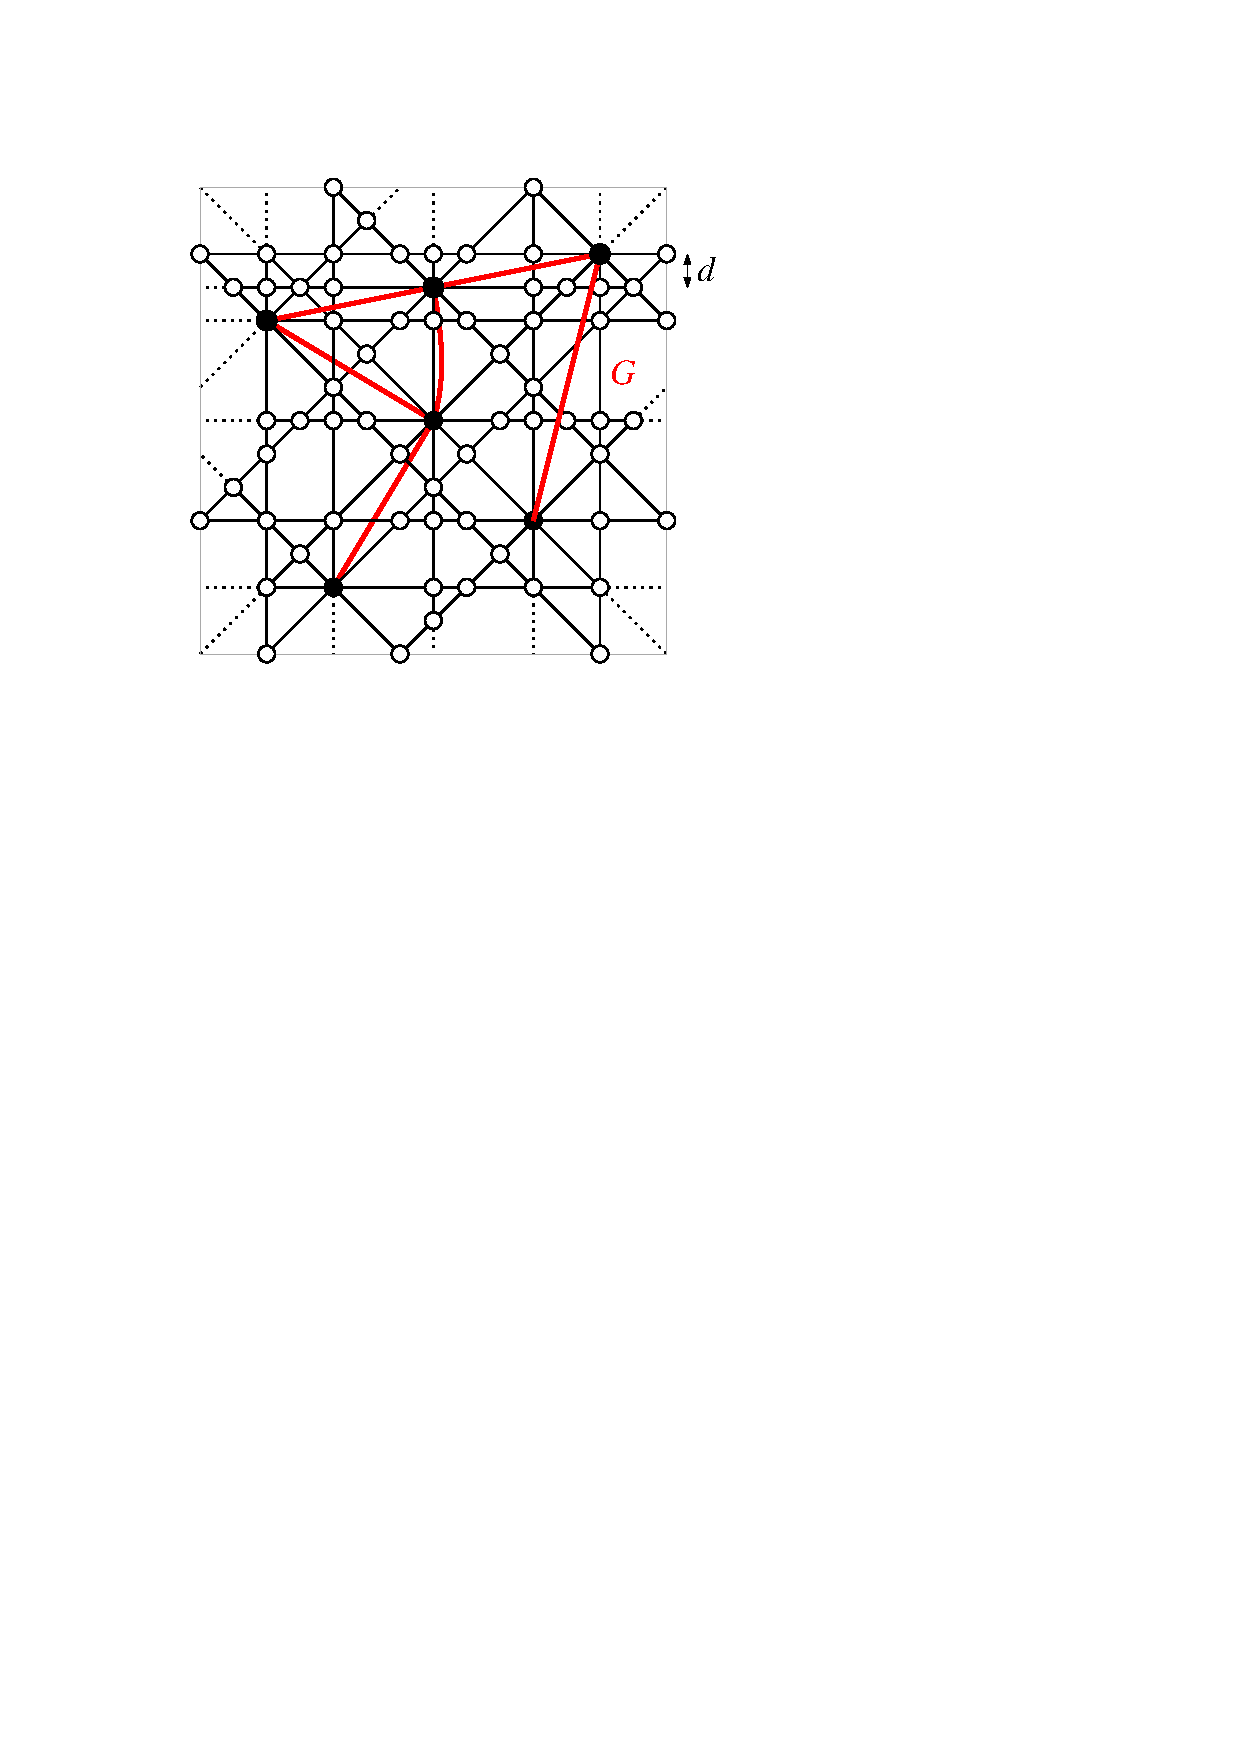
\includegraphics[width=0.24\textwidth]{figures2/node.pdf}
	\hfill
	\includegraphics[width=0.2257\textwidth,trim=0 0 15 0, clip, page=2]{figures2/node.pdf}
	\caption{Left: a bounding-box restricted octilinear Hanan grid for an input graph $G$. All depicted nodes are part of $O(G)$, but only the black nodes were part of the input graph $G$ and have been snapped to a base grid with cell size $d$ prior to construction of $O(G)$. Edges of $G$ are depicted in red. Right: an octilinear drawing of $G$ on $O(G)$.}
	\label{FIG:octihanangrid}
	\vspace{-.65cm}
\end{figure}

As rectilinear Metro Maps are of only little interest, we slightly extend the definition of a classic Hanan grid and introduce the concept of octilinear Hanan grids.
Given a point set $P$ on the plane, the construction of an octilinear Hanan grid $O(P)$ is similar to a classic Hanan grid, but we also draw diagonal lines and consider them for possible intersection points.
Obviously, all paths in $O(P)$ will only consist of segments with an octilinear orientation.

\subsection{Base Grid Snapping}

As we would like to maintain a minimum segment length in the final maps, we do not construct the octilinear Hanan grid directly on the input graph $G$, but first snap its node positions to a regular base grid.

\subsection{Hanan Iterations}

An octilinear Hanan grid $O(P)$ with nodes $V$ can be made increasingly more fine-grained if we take the nodes $V$ as points $P'$ and construct an octilinear Hanan grid $O(P')$ from them.
We call such a step a Hanan iteration.

\TODO{Show example iterations}

\subsection{Path Cost Preserving Weights}

\section{Quad-Tree}

A quad tree is a grid which can be constructed for a set $P$ of input points in the following way: start with the bounding box of $P$ as a single-cell grid.
While any cell has more points in it than a threshold value $t$, split this cell into 4 rectangular cells.
The resulting grid has a graph-like structure, where each grid cell of size $d$ may have 4 direct child vertices of size $d / 2$.

\section{Ortho-Radial Grid}

Recent work discussed the problem of drawing Metro Maps in an ortho-radial fashion \cite{TODO}.
While octilinear Metro Maps are much more common than ortho-radial maps, the latter can still be found and have an intriguing visual quality \TODO{example}.
In \cite{TODO}, it was observed that an ortho-radial map can be understood as a flat projection of an octilinear map which is joined at two parallel sides.
Figure~\ref{FIG:orthoradgrid}, left depicts a classic ortho-radial grid graph.
An obvious problem with such a grid are the large white-space areas, as the grid cell size grows with increasing distance to the grid center.
To overcome this, we use a slightly altered ortho-radial grid graph, as depicted in Figure~\ref{FIG:orthoradgrid}, right.
The innermost ring starts with a number of nodes $b = 8$, but this number is doubled each time the ring radius doubles.
So at ring 1, $b_1 = 8$, at ring 2, $b_2 = 16$, $b_4 = 32$, $b_8 = 64$ and so on.
This will give our maps a denser look while still maintaining the visual impression or ortho-radiality.

\begin{figure}
    \centering
	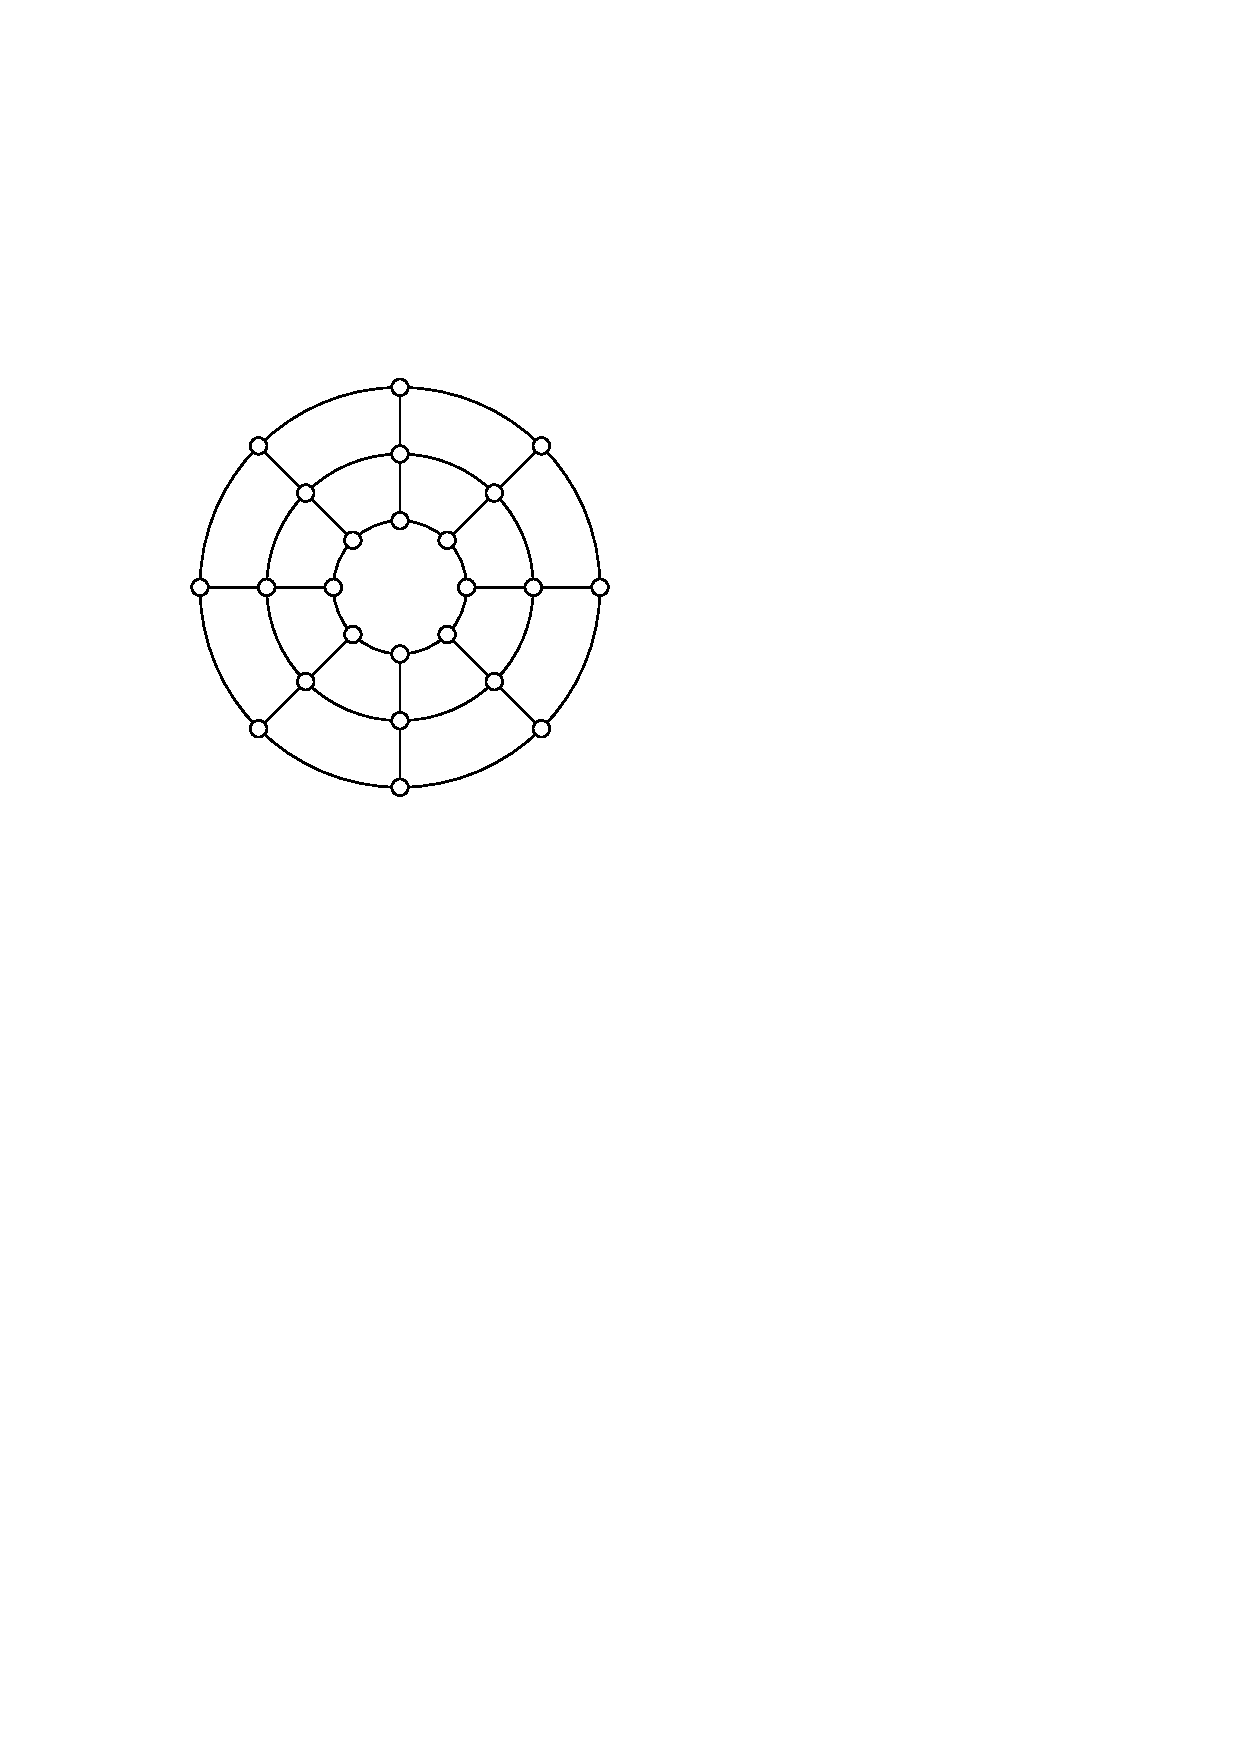
\includegraphics[width=0.23\textwidth]{figures2/ortho.pdf}
	\hfill
	\includegraphics[width=0.23\textwidth,page=2]{figures2/ortho.pdf}
	\caption{Two kinds of ortho-radial grid graphs. Left: Ortho-radial grid graph with $b = 8$ and a central node. Right: Ortho-radial grid graph where $b$ is doubled each time the radius doubles.}
	\label{FIG:orthoradgrid}
\end{figure}

\section{Experimental Evaluation}

\subsection{Effect of Octilinear Hanan Grid on Solution Times and Quality}

\subsection{Effect of Quad Trees on Solution Times and Quality}

\subsection{Ortho-Radial Experiments}

\section{Conclusion and Future Work}

\TODO{Mention local enlargement prior to ortho-radial drawing}

\bibliographystyle{ACM-Reference-Format}
\bibliography{pfaedle}
\end{document}
